\documentclass[../main]{subfiles}
\begin{document}

\chapter{正交相干检波器}%
\label{cha:iq}

\section{实验报告}%
\label{sec:\arabic{chapter}report}

\begin{Exercise}
  记录波形、测试数据并填入表格。
\end{Exercise}

\begin{Answer}
  \begin{itemize}
    \item 波形见图~\ref{fig:iq}。
    \item 仿真波形见图~\ref{fig:iq_}。
    \item 测试数据见表~\ref{tab:sin}和表~\ref{tab:phase}。
    \item 仿真代码见程序~\ref{lst:iq}。
  \end{itemize}
\end{Answer}

\begin{figure}[htbp]
  \centering
  \begin{subfigure}[htbp]{0.45\linewidth}
    \centering
    \includegraphics[
      width = \linewidth,
    ]{images/iq.png}
    \caption{同相正交信号}%
    \label{fig:_iq}
  \end{subfigure}
  \quad
  \begin{subfigure}[htbp]{0.45\linewidth}
    \centering
    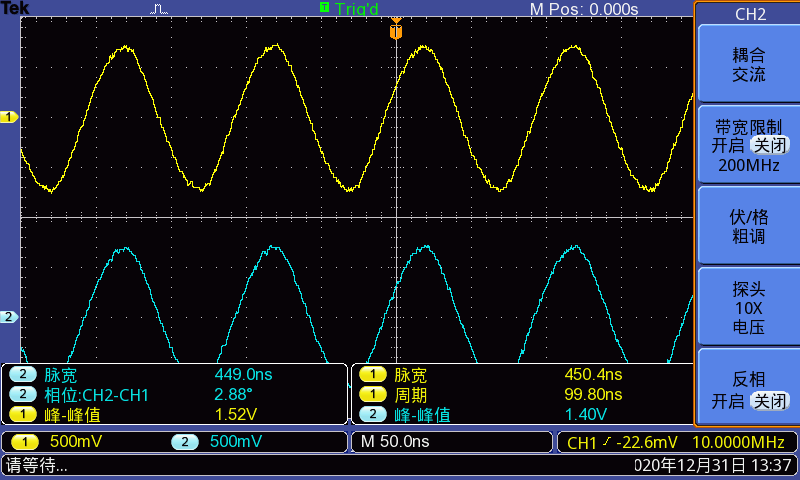
\includegraphics[
      width = \linewidth,
    ]{images/f.png}
    \caption{中频}%
    \label{fig:f}
  \end{subfigure}
  \caption{正交相干检波器}%
  \label{fig:iq}
\end{figure}

\begin{figure}[htbp]
  \centering
  \includegraphics[
    width = 0.8\linewidth,
  ]{figures/iq.pdf}
  \caption{以输入频率 9.6 MHz 为例。 $s$ 为滤波前信号, $r$ 为滤波后信号}%
  \label{fig:iq_}
\end{figure}

\begin{table}[htbp]
  \centering
  \caption{改变 sin 输入频率}%
  \label{tab:sin}
  \tiny
  \csvautobooktabular[respect percent]{tables/sin.csv}
\end{table}

\begin{table}[htbp]
  \centering
  \caption{测试中频本振的幅相不平衡度}%
  \label{tab:phase}
  \csvautobooktabular[respect percent]{tables/phase.csv}
\end{table}

\langCVfile[matlab][lst:iq][matlab]{figures/iq.m}{figures/iq.m}

\begin{Exercise}
  分析实验过程中出现的问题和现象。
\end{Exercise}

\begin{Answer}
  如表~\ref{tab:sin}所示,由于乘法器的外差原理,输出频率一定是本振频率与输入
  频率之差。由于本振的幅相不平衡度,同相正交信号也不会是理想的频率相等、完全
  正交的两路正弦波。
\end{Answer}

\begin{Exercise}
  实验报告中完成思考题。
\end{Exercise}

\begin{Answer}
  见章节~\ref{sec:\arabic{chapter}thought}。
\end{Answer}

\section{实验思考}%
\label{sec:\arabic{chapter}thought}

\begin{Exercise}
  幅相不平衡是什么原因造成的?
\end{Exercise}

\begin{Answer}
  \begin{itemize}
    \item 移相器非理想。
    \item 正交、同相支路的乘法器、低通滤波器不可能做到完全一致。
    \item 外界温度、噪声。
  \end{itemize}
\end{Answer}

\begin{Exercise}
  幅相不平衡如何进行调整?
\end{Exercise}

\begin{Answer}
  采用误差校正技术。在检波前输入一个已知信号,输出信号反映幅相不平衡,以此来
  校正误差。
\end{Answer}

\begin{Exercise}
  不同频率下为什么幅相不平衡度不一致?
\end{Exercise}

\begin{Answer}
  乘法器是有源器件,在不同频率下输出信号偏差不一样,所以不同频率下幅相不平衡
  度不一致。
\end{Answer}

\end{document}
